\documentclass{standalone}
\usepackage{tikz}
\usetikzlibrary{patterns, positioning}


\begin{document}
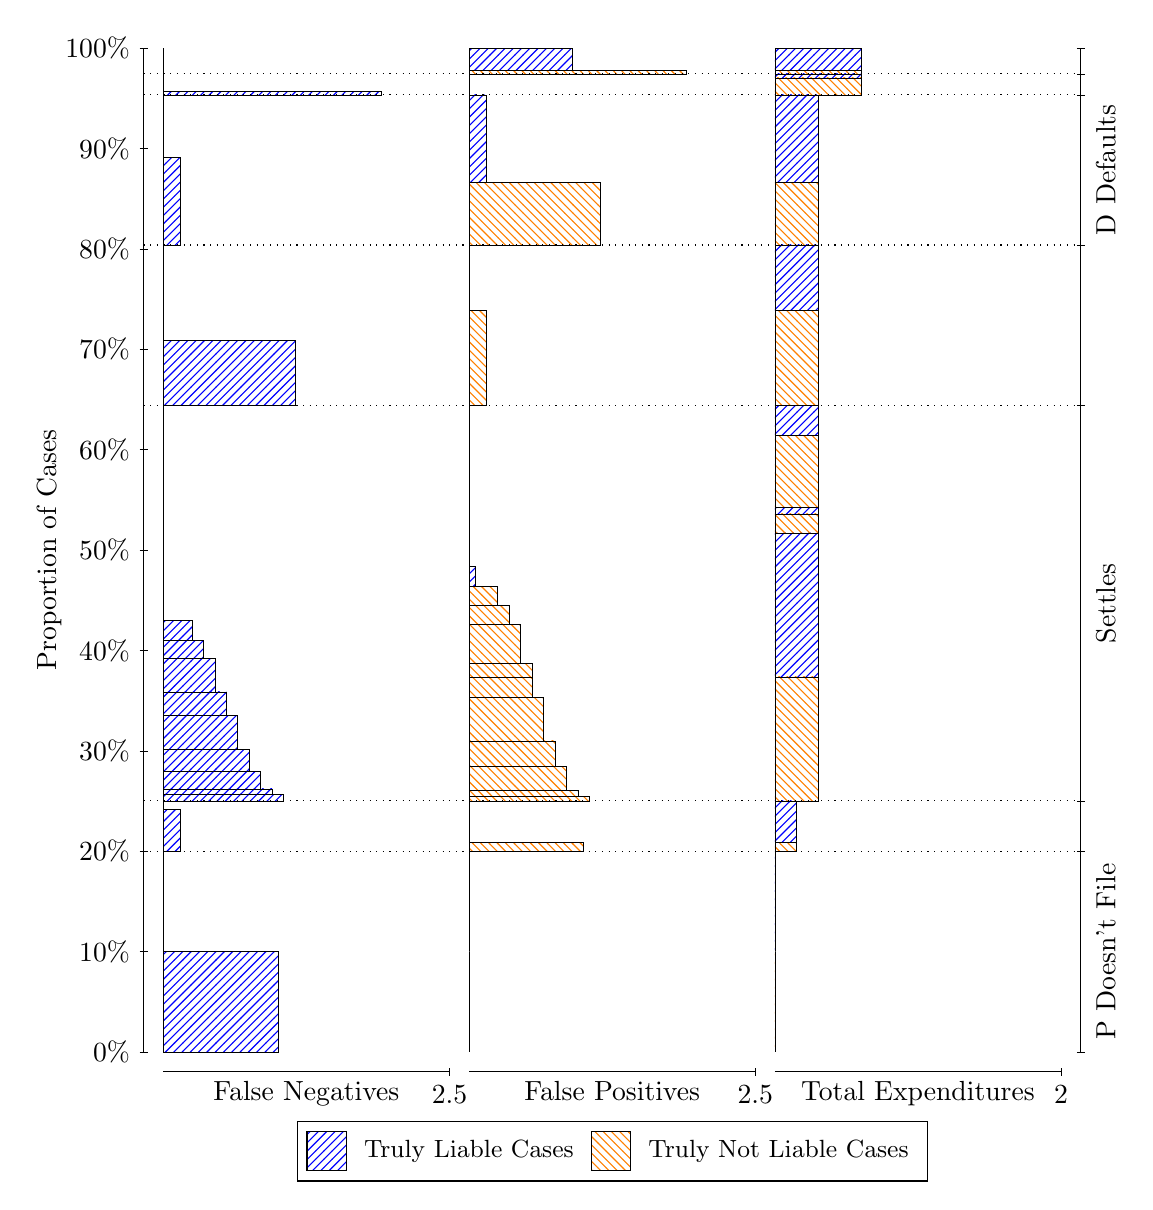
\begin{tikzpicture}
\draw[black, very thin] (1.5,1.75) -- (1.5,14.5);
\node[rotate=90, text=black, anchor=center] at (0.3, 8.125) {Proportion of Cases};
\draw[black, very thin] (1.45,1.75) -- (1.55,1.75);
\node[text=black, anchor=east] at (1.45, 1.75) {0\%};
\draw[black, very thin] (1.45,3.025) -- (1.55,3.025);
\node[text=black, anchor=east] at (1.45, 3.025) {10\%};
\draw[black, very thin] (1.45,4.3) -- (1.55,4.3);
\node[text=black, anchor=east] at (1.45, 4.3) {20\%};
\draw[black, very thin] (1.45,5.575) -- (1.55,5.575);
\node[text=black, anchor=east] at (1.45, 5.575) {30\%};
\draw[black, very thin] (1.45,6.85) -- (1.55,6.85);
\node[text=black, anchor=east] at (1.45, 6.85) {40\%};
\draw[black, very thin] (1.45,8.125) -- (1.55,8.125);
\node[text=black, anchor=east] at (1.45, 8.125) {50\%};
\draw[black, very thin] (1.45,9.4) -- (1.55,9.4);
\node[text=black, anchor=east] at (1.45, 9.4) {60\%};
\draw[black, very thin] (1.45,10.675) -- (1.55,10.675);
\node[text=black, anchor=east] at (1.45, 10.675) {70\%};
\draw[black, very thin] (1.45,11.95) -- (1.55,11.95);
\node[text=black, anchor=east] at (1.45, 11.95) {80\%};
\draw[black, very thin] (1.45,13.225) -- (1.55,13.225);
\node[text=black, anchor=east] at (1.45, 13.225) {90\%};
\draw[black, very thin] (1.45,14.5) -- (1.55,14.5);
\node[text=black, anchor=east] at (1.45, 14.5) {100\%};

\draw[black, very thin] (13.4,1.75) -- (13.4,14.5);
\draw[black, very thin] (13.35,1.75) -- (13.45,1.75);
\node[anchor=west] at (13.35, 1.75) {};
\draw[black, very thin] (13.35,4.3) -- (13.45,4.3);
\node[anchor=west] at (13.35, 4.3) {};
\draw[black, very thin] (13.35,4.9397) -- (13.45,4.9397);
\node[anchor=west] at (13.35, 4.9397) {};
\draw[black, very thin] (13.35,9.958) -- (13.45,9.958);
\node[anchor=west] at (13.35, 9.958) {};
\draw[black, very thin] (13.35,11.999) -- (13.45,11.999);
\node[anchor=west] at (13.35, 11.999) {};
\draw[black, very thin] (13.35,13.905) -- (13.45,13.905);
\node[anchor=west] at (13.35, 13.905) {};
\draw[black, very thin] (13.35,14.171) -- (13.45,14.171);
\node[anchor=west] at (13.35, 14.171) {};
\draw[black, very thin] (13.35,14.5) -- (13.45,14.5);
\node[anchor=west] at (13.35, 14.5) {};

\draw[black, very thin, pattern color=blue, pattern=north east lines] (1.75,1.75) rectangle (3.2033,3.025);
\draw[black, very thin, pattern color=orange, pattern=north west lines] (1.75,3.025) rectangle (1.75,4.3);
\draw[black, very thin, pattern color=blue, pattern=north east lines] (1.75,4.3) rectangle (1.968,4.8296);
\draw[black, very thin, pattern color=orange, pattern=north west lines] (1.75,4.8296) rectangle (1.75,4.9397);
\draw[black, very thin, pattern color=blue, pattern=north east lines] (1.75,4.9397) rectangle (3.276,5.0247);
\draw[black, very thin, pattern color=blue, pattern=north east lines] (1.75,5.0247) rectangle (3.1307,5.0919);
\draw[black, very thin, pattern color=blue, pattern=north east lines] (1.75,5.0919) rectangle (2.9853,5.315);
\draw[black, very thin, pattern color=blue, pattern=north east lines] (1.75,5.315) rectangle (2.84,5.5937);
\draw[black, very thin, pattern color=blue, pattern=north east lines] (1.75,5.5937) rectangle (2.6947,6.0241);
\draw[black, very thin, pattern color=blue, pattern=north east lines] (1.75,6.0241) rectangle (2.5493,6.3232);
\draw[black, very thin, pattern color=blue, pattern=north east lines] (1.75,6.3232) rectangle (2.404,6.7511);
\draw[black, very thin, pattern color=blue, pattern=north east lines] (1.75,6.7511) rectangle (2.2587,6.9815);
\draw[black, very thin, pattern color=blue, pattern=north east lines] (1.75,6.9815) rectangle (2.1133,7.236);
\draw[black, very thin, pattern color=orange, pattern=north west lines] (1.75,7.236) rectangle (1.75,9.958);
\draw[black, very thin, pattern color=blue, pattern=north east lines] (1.75,9.958) rectangle (3.4213,10.79);
\draw[black, very thin, pattern color=orange, pattern=north west lines] (1.75,10.79) rectangle (1.75,11.999);
\draw[black, very thin, pattern color=blue, pattern=north east lines] (1.75,11.999) rectangle (1.968,13.112);
\draw[black, very thin, pattern color=orange, pattern=north west lines] (1.75,13.112) rectangle (1.75,13.905);
\draw[black, very thin, pattern color=blue, pattern=north east lines] (1.75,13.905) rectangle (4.5113,13.954);
\draw[black, very thin, pattern color=orange, pattern=north west lines] (1.75,13.954) rectangle (1.75,14.171);
\draw[black, very thin, pattern color=orange, pattern=north west lines] (1.75,14.171) rectangle (1.75,14.22);
\draw[black, very thin, pattern color=blue, pattern=north east lines] (1.75,14.22) rectangle (1.75,14.5);
\draw[black, very thin, pattern color=orange, pattern=north west lines] (5.6333,1.75) rectangle (5.6333,3.025);
\draw[black, very thin, pattern color=blue, pattern=north east lines] (5.6333,3.025) rectangle (5.6333,4.3);
\draw[black, very thin, pattern color=orange, pattern=north west lines] (5.6333,4.3) rectangle (7.0867,4.4101);
\draw[black, very thin, pattern color=blue, pattern=north east lines] (5.6333,4.4101) rectangle (5.6333,4.9397);
\draw[black, very thin, pattern color=orange, pattern=north west lines] (5.6333,4.9397) rectangle (7.1593,4.9912);
\draw[black, very thin, pattern color=orange, pattern=north west lines] (5.6333,4.9912) rectangle (7.014,5.0738);
\draw[black, very thin, pattern color=orange, pattern=north west lines] (5.6333,5.0738) rectangle (6.8687,5.3801);
\draw[black, very thin, pattern color=orange, pattern=north west lines] (5.6333,5.3801) rectangle (6.7233,5.7009);
\draw[black, very thin, pattern color=orange, pattern=north west lines] (5.6333,5.7009) rectangle (6.578,6.254);
\draw[black, very thin, pattern color=orange, pattern=north west lines] (5.6333,6.254) rectangle (6.4327,6.5129);
\draw[black, very thin, pattern color=orange, pattern=north west lines] (5.6333,6.5129) rectangle (6.4327,6.6873);
\draw[black, very thin, pattern color=orange, pattern=north west lines] (5.6333,6.6873) rectangle (6.2873,7.1833);
\draw[black, very thin, pattern color=orange, pattern=north west lines] (5.6333,7.1833) rectangle (6.142,7.4222);
\draw[black, very thin, pattern color=orange, pattern=north west lines] (5.6333,7.4222) rectangle (5.9967,7.6617);
\draw[black, very thin, pattern color=blue, pattern=north east lines] (5.6333,7.6617) rectangle (5.706,7.9163);
\draw[black, very thin, pattern color=blue, pattern=north east lines] (5.6333,7.9163) rectangle (5.6333,9.958);
\draw[black, very thin, pattern color=orange, pattern=north west lines] (5.6333,9.958) rectangle (5.8513,11.167);
\draw[black, very thin, pattern color=blue, pattern=north east lines] (5.6333,11.167) rectangle (5.6333,11.999);
\draw[black, very thin, pattern color=orange, pattern=north west lines] (5.6333,11.999) rectangle (7.3047,12.792);
\draw[black, very thin, pattern color=blue, pattern=north east lines] (5.6333,12.792) rectangle (5.8513,13.905);
\draw[black, very thin, pattern color=orange, pattern=north west lines] (5.6333,13.905) rectangle (5.6333,14.122);
\draw[black, very thin, pattern color=blue, pattern=north east lines] (5.6333,14.122) rectangle (5.6333,14.171);
\draw[black, very thin, pattern color=orange, pattern=north west lines] (5.6333,14.171) rectangle (8.3947,14.22);
\draw[black, very thin, pattern color=blue, pattern=north east lines] (5.6333,14.22) rectangle (6.9413,14.5);
\draw[black, very thin, pattern color=orange, pattern=north west lines] (9.5167,1.75) rectangle (9.5167,3.025);
\draw[black, very thin, pattern color=blue, pattern=north east lines] (9.5167,3.025) rectangle (9.5167,4.3);
\draw[black, very thin, pattern color=orange, pattern=north west lines] (9.5167,4.3) rectangle (9.7892,4.4101);
\draw[black, very thin, pattern color=blue, pattern=north east lines] (9.5167,4.4101) rectangle (9.7892,4.9397);
\draw[black, very thin, pattern color=orange, pattern=north west lines] (9.5167,4.9397) rectangle (10.062,6.5129);
\draw[black, very thin, pattern color=blue, pattern=north east lines] (9.5167,6.5129) rectangle (10.062,8.3435);
\draw[black, very thin, pattern color=orange, pattern=north west lines] (9.5167,8.3435) rectangle (10.062,8.5831);
\draw[black, very thin, pattern color=blue, pattern=north east lines] (9.5167,8.5831) rectangle (10.062,8.668);
\draw[black, very thin, pattern color=orange, pattern=north west lines] (9.5167,8.668) rectangle (10.062,9.5773);
\draw[black, very thin, pattern color=blue, pattern=north east lines] (9.5167,9.5773) rectangle (10.062,9.958);
\draw[black, very thin, pattern color=orange, pattern=north west lines] (9.5167,9.958) rectangle (10.062,11.167);
\draw[black, very thin, pattern color=blue, pattern=north east lines] (9.5167,11.167) rectangle (10.062,11.999);
\draw[black, very thin, pattern color=orange, pattern=north west lines] (9.5167,11.999) rectangle (10.062,12.792);
\draw[black, very thin, pattern color=blue, pattern=north east lines] (9.5167,12.792) rectangle (10.062,13.905);
\draw[black, very thin, pattern color=orange, pattern=north west lines] (9.5167,13.905) rectangle (10.607,14.122);
\draw[black, very thin, pattern color=blue, pattern=north east lines] (9.5167,14.122) rectangle (10.607,14.171);
\draw[black, very thin, pattern color=orange, pattern=north west lines] (9.5167,14.171) rectangle (10.607,14.22);
\draw[black, very thin, pattern color=blue, pattern=north east lines] (9.5167,14.22) rectangle (10.607,14.5);
\draw[black, dotted] (1.5,4.3) -- (13.4,4.3);
\draw[black, dotted] (1.5,4.9397) -- (13.4,4.9397);
\draw[black, dotted] (1.5,9.958) -- (13.4,9.958);
\draw[black, dotted] (1.5,11.999) -- (13.4,11.999);
\draw[black, dotted] (1.5,13.905) -- (13.4,13.905);
\draw[black, dotted] (1.5,14.171) -- (13.4,14.171);
\draw[black, very thin] (1.75,1.5) -- (5.3833,1.5);
\node[text=black, anchor=north] at (3.5667, 1.5) {False Negatives};
\draw[black, very thin] (5.3833,1.45) -- (5.3833,1.55);
\node[text=black, anchor=north] at (5.3833, 1.45) {2.5};

\draw[black, very thin] (5.6333,1.5) -- (9.2667,1.5);
\node[text=black, anchor=north] at (7.45, 1.5) {False Positives};
\draw[black, very thin] (9.2667,1.45) -- (9.2667,1.55);
\node[text=black, anchor=north] at (9.2667, 1.45) {2.5};

\draw[black, very thin] (9.5167,1.5) -- (13.15,1.5);
\node[text=black, anchor=north] at (11.333, 1.5) {Total Expenditures};
\draw[black, very thin] (13.15,1.45) -- (13.15,1.55);
\node[text=black, anchor=north] at (13.15, 1.45) {2};

\node[text=black, centered, rotate=90] at (13.72, 3.025) {P Doesn't File};

\node[text=black, centered, rotate=90] at (13.72, 7.4489) {Settles};

\node[text=black, centered, rotate=90] at (13.72, 12.952) {D Defaults};



\draw (7.449999999999999,1.5) node[draw=none] (baseCoordinate) {};
\begin{scope}[align=center]
        \matrix[scale=0.5, draw=black, below=0.5cm of baseCoordinate, nodes={draw}, column sep=0.1cm]{
            \node[rectangle, draw, minimum width=0.5cm, minimum height=0.5cm, pattern color=blue, pattern=north east lines] {}; &
            \node[draw=none, font=\small, text=black] (B) {Truly Liable Cases}; &
            \node[rectangle, draw, minimum width=0.5cm, minimum height=0.5cm, pattern color=orange, pattern=north west lines] {}; &
            \node[draw=none, font=\small, text=black] (B) {Truly Not Liable Cases}; \\
            };
\end{scope}

\end{tikzpicture}
\end{document}